%% This is the impactor chapter for my UBC PhD Dissertation
%% The parent document is called thesis.tex

\chapter{Design of a fall simulator}
\label{ch:fall_sim_design}
Before the behaviour of the proximal in a simulated fall can be compared to the behaviour in quasi-static loading, a validated impact fall simulator must be developed.
Impact fall simulation has been used by the hip protector design community for many years, however, the particular requirements of testing human material makes adaptation of a pre-existing fall simulator impossible.
In this chapter, the rational, design and justification for a drop tower apparatus that simulates a human fall to the side from standing, is presented.

This chapter was published as a peer reviewed paper in ASME Journal of Biomechanical Engineering~\citep{gilchrist_development_2013} and is reprinted here with permission.

\section{Introduction}
\label{sec:fall_sim_design_intro}
Hip fracture is a devastating injury associated with high morbidity and mortality in the elderly as well as high treatment cost~\citep{braithwaite_estimating_2003, forsen_survival_1999,wiktorowicz_economic_2001}.
In order to prevent or improve treatment of these injuries, researchers have conducted extensively laboratory studies, with previous \textit{ex vivo} models of hip fracture establishing the role of posture~\citep{pinilla_impact_1996, ford_effect_1996}, compression rate~\citep{courtney_effects_1994, weber_proximal_1992}, and bone density~\citep{lotz_use_1990, lochmuller_mechanical_2002, manske_cortical_2008} in the strength of the femur.
Bone density has been shown to correlate to the strength of a proximal femur loaded in a fall posture, and constant compression rates ranging from 0.7~\ac{mm}/\ac{s}~ to 100~\ac{mm}/\ac{s}~\citep{courtney_effects_1994, weber_proximal_1992} have been used to prove that the proximal femur's mechanical properties depend on compression rate magnitude.

In all of the previous studies, tests were conducted using materials testing machines to apply loads to either the head or lateral trochanter of the femur~\citep{boehm_prediction_2008, courtney_effects_1994, de_bakker_during_2009, lochmuller_mechanical_2002, lotz_use_1990, manske_cortical_2008, roberts_comparison_2010, weber_proximal_1992, keyak_relationships_2000}.
While compression rate varied from experiment to experiment, in each case it was fixed and constant throughout testing, and the final result was fracture of the bone.
Only two researchers have conducted tests at high compression rates~\citep{weber_proximal_1992, backman_proximal_1957}, potentially representative of rates that would be experienced in a fall, but they tested the femur in isolation, neglecting the influence of surrounding tissues and structures.

Falls are by definition dynamic, inertia-driven events in which compression rates are not constant, and in some portions of the event may be as high as 3000~\ac{mm}/\ac{s}~\citep{feldman_reducing_2007}, although in individuals that are able to react quickly, fall speeds are often slowed due to an extended hand or other protective action~\citep{van_den_kroonenberg_dynamic_1995, feldman_reducing_2007}.
Additionally, fracture is not prescribed in a fall, with only $ \sim $5\% of falls resulting in fracture~\citep{nachreiner_circumstances_2007}.
In a fall to the side, the compression rate of the proximal femur is dependent on the contact velocity with the ground, properties of the overlying soft tissue, stiffness and mass of the pelvis, mass of the body, and the stiffness of the proximal femur itself.
The stiffness of the proximal femur is of primary importance to its resulting behaviour and is itself a function of compression (strain) rate~\citep{mcelhaney_dynamic_1966, crowninshield_response_1974, saha_instrumented_1974, currey_effects_1975, carter_bone_1976, robertson_compressive_1978, linde_mechanical_1991, courtney_effects_1994, pithioux_comparison_2004, hansen_effect_2008, zioupos_microcracking_2008, weber_proximal_1992}.
The recursive nature of this process means that the compression rate of the femur will not be constant during the impact event and in only a subset of bones will result in fracture.
Modelling the compression rate of the lateral femur as a constant, and deterministically imposing fracture, is a significant limitation of the previous experiments, and may limit their ability to inform researchers about the mechanics of the fracture and how to identify the specific bones that are susceptible to fracture.

In addition to these biomechanical observations, epidemiological research has shown that a discrepancy exists between what is expected from lab results and what is seen in the general population.
Lab and epidemiology results~\citep{borissova_femoral_2011, cauley_risk_2009} have shown that bone density is an important factor that is correlated to fracture load, but we also see that more than two-thirds of fractures occur outside the low bone density population~\citep{stone_bmd_2003, siris_bone_2004, greenspan_fall_1994}
This indicates that other factors (\ac{eg}, structural) may be involved~\citep{singh_changes_1970, naylor_use_2012, bouxsein_bone_2003}.

No researchers have explicitly modelled the fall and observed the resulting bone behaviour, which would dependent recursively on both fall mechanics and the bone's response, as described above.
Understanding these behaviours may illuminate potential screening targets, helping inform and improve biomechanical (\ac{eg}, hip protectors) and clinical (\ac{eg}, pharmaceutical) hip fracture prevention.
Thus, in an effort to bridge the gap between current \textit{ex vivo} hip fracture models and \textit{in vivo} fractures, this research comprises two related aims: a) develop an impact-based testing apparatus to model a physiological fall to the side, including representations of the surrounding anatomic structures; b) validate quantitative methods for analysing loading mechanics using high speed imaging and surface strain analysis.

The mechanics of hip fracture are influenced by the structures and tissues (referred to as \emph{elements}) surrounding the femur.
These elements are, on the medial side, the pelvis and body, and on the lateral side, the soft tissue over the trochanter.
Previous efforts have been made to understand the behaviour of these elements in isolation, and in some cases researchers have incorporated them into tests to evaluate the effectiveness of biomechanical devices such as hip protectors or compliant flooring~\citep{robinovitch_hip_2009, laing_force_2008,laing_effect_2006}.
In the following sections, research surrounding each element will be considered and representative properties will be chosen for inclusion in our laboratory model.
Finally, the behaviour of the model during a simulated fall will be compared to the behaviour of published human volunteer tests to evaluate the biofidelity of the apparatus.

In addition to the above device development, a quantitative method of evaluating the strain on the bone surface will be validated.
Researchers have traditionally used strain gauges to evaluate the strain state of the proximal femur during loading to fracture~\citep{cristofolini_vitro_2007}.
It is known from finite element analyses~\citep{verhulp_comparison_2006} and from research on the experimental error of strain gauges~\citep{cristofolini_vitro_1997} that strain gradients on bones can be high.
This has two primary consequences for their use for strain measurement: 1) it is difficult to compare two models of the same event (\ac{eg}, comparing a fracture experiment to a subject-specific finite element model), and 2) placement of gauges in locations where meaningful strain is "guaranteed" to occur is impossible.
In an experiment complementary to the development of the fall simulator, we will directly compare strain measurements from \acf{dic}, which is a method for full field strain measurement, to the gold standard strain rosette.
Our goal is to validate the use of \ac{dic} for measurement of strain on the surface of a proximal femur so that future experiments can use it in lieu of strain rosettes.

\section{Materials and methods}
\label{sec:fall_sim_design_methods}
A drop tower-based fall simulation apparatus was developed and its loading mechanics were compared to the response of volunteer, as well as human cadaver hip and pelvis tests.
In addition to the apparatus development, low compression rate, sub-failure tests were conducted on human bone specimens to validate the use of digital image correlation for surface strain measurement on the femoral neck.
These techniques will be used in future experiments to determine the loading and fracture mechanics of human proximal femora loaded in a fall configuration.

	\subsection{Fall simulator apparatus}
	\label{sec:fall_sim_design_methods_apparatus}
	Due to the dynamic nature of a fall to the side, the tissues and structures surrounding the proximal femur must be included for accurate biofidelic modelling.
	These structures are, on the lateral side of the femur, skin and soft tissue over the trochanter, and on the medial side, the pelvis and body.
	The biological scenario was simplified to a lumped parameter model (Figure \ref{fig:MassModel}) which was characterized using a state-of-the-art plastic bone surrogate for consistency (3rd Gen.\ Large Femur, Sawbones\texttrademark, Vashon, WA).
	The following sections contain a literature review and justification for the properties selected for each element.
	
	\begin{figure}
		\centering
		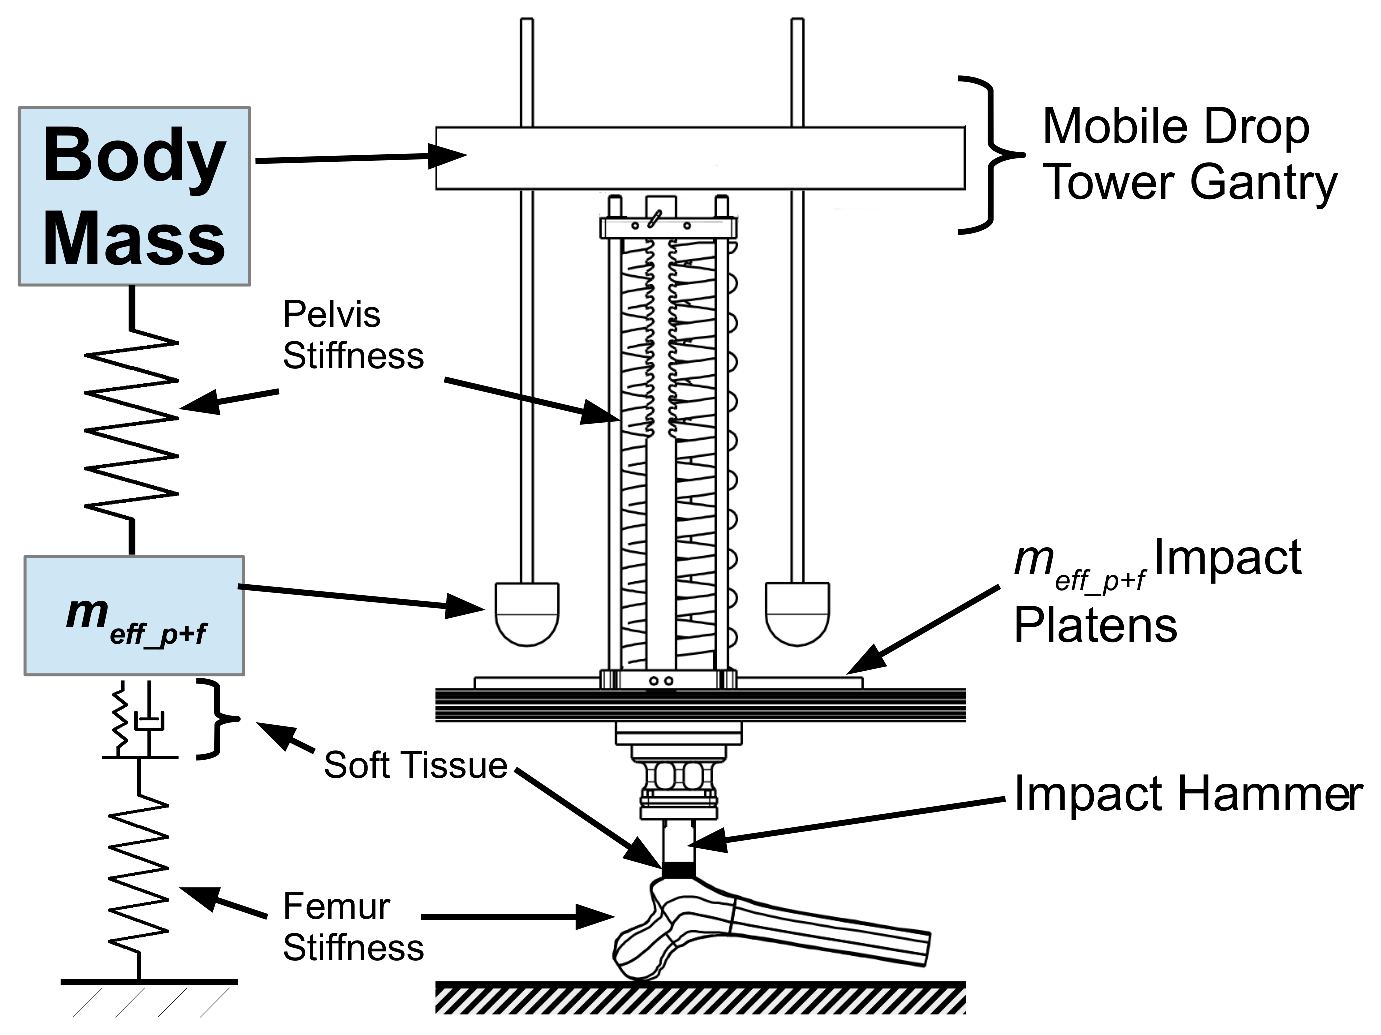
\includegraphics[width=.7\linewidth]{./impactor/figures/MassModel.eps}
		\caption[Schematic of the fall simulator]{\textbf{Schematic of the fall simulator showing the mass and spring of structures that influence loading a fall to the side.
		$m_{eff\_p+f}$ is the effective mass of the lateral pelvis and femur.}}
		\label{fig:MassModel}
	\end{figure}

		\subsubsection{Effective body mass}
		\label{sec:fall_sim_design_methods_apparatus_body}
		The selection of the body mass determines (along with the pelvis and soft tissue stiffnesses) the peak force and (along with the impact velocity) the energy delivered during the impact.
		Body habitus, measured using BMI, has been shown to correlate negatively with hip fracture risk~\citep{orwoll_finite_2009, parker_association_2008, nguyen_abdominal_2005, nguyen_identification_2005, minns_are_2007}, indicating that increased body mass can be protective.
		There is, however, also some evidence to the contrary, especially that very high body mass can increase fracture risk~\citep{nielson_bmi_2011}.
		To quantify how body mass influences the loading parameters during a fall, researchers have mathematically modelled falls using link assemblies~\citep{van_den_kroonenberg_dynamic_1995}, and performed pelvis drop experiments on young, university-student volunteers~\citep{robinovitch_prediction_1991, laing_characterizing_2010}.
		
		In a fall to the side the effective body mass impacting the trochanter is less than the total body mass of the person falling.
		Conceptually, this is because some of the body mass would be supported by the feet and lower extremities.
		Experimentalists and computational modellers have put this so-called \emph{effective body mass} at approximately half body weight~\citep{van_den_kroonenberg_dynamic_1995, robinovitch_prediction_1991}.
		Additionally, direct measurement of the effective mass in young volunteers has provided a range of 24.1--50~\ac{kg}~\citep{robinovitch_prediction_1991, van_den_kroonenberg_dynamic_1995, robinovitch_distribution_1997, laing_force_2008} with a cross-study average for human tests subjects of 31.9~\ac{kg}.
		The cross-study average for the computational models was higher, and more variable depending on the assumptions made in the model.
		The cross-study average of human subjects did not show the same variability due to model design, or dependency on assumptions, and was taken as the value of the effective body mass.
		A value of 32~\ac{kg} was selected for the fall simulator, which is within one standard deviation of 50\% body weight of hip fracture cases~\citep{armstrong_body_2011, orwoll_finite_2009, bouxsein_contribution_2007, nielson_trochanteric_2009}.

		\subsubsection{Effective mass of the femur and lateral pelvis}
		\label{sec:fall_sim_design_methods_apparatus_pelvis}
		The two main mass components that govern the loading of the proximal femur in a fall are: a) the body mass, whose impact is attenuated by the compliance of the pelvis, and the selection of which was discussed above; and b) the mass of the lateral pelvis and proximal femur, whose impact is attenuated only by the compliance of the femur and overlying soft tissue (Figure \ref{fig:MassModel}).
		Previous work on pelvis fracture in automotive, side-impact accidents performed impacts of osteoligamentous pelvises at $\sim$4.5~\ac{m}/\ac{s}~\citep{beason_bone_2003}.
		In these experiments, an impact hammer was instrumented with a load cell and dropped on to the greater trochanter of the femur.
		In the resulting force-time traces a force spike was seen early in the loading history, before deformation of the pelvis started (Figure \ref{fig:CompBeason}).
		This force spike was created by the inertia of the mass close to the impact surface.
		
		To better understand the origin of this pulse, consider that in an impact, the velocity of the impact hammer and the contact point on the object being impacted must become equal, creating a force due to the inertia of the mass near the contact point.
		In the case of a fall to the side, before the pelvis can compress, the proximal femur and lateral pelvis must go from moving 3~\ac{m}/\ac{s}, to being stationary against the ground.
		This happens very quickly, requiring a high acceleration, and creating a force pulse at the interface between the ground and the trochanter.
		This behaviour has been documented in head-first impact studies, where a force pulse is generated as the head is stopped before compression of the neck begins \citep{nightingale_dynamic_1997, saari_cervical_2011}.
		In the fall to the side, as one moves medially from the contact point, the pulse is attenuated due to the compliance of the tissues between the ground and the location under consideration.
		Because they are relatively stiff and close to the impact surface, the lateral trochanter and femoral neck will see a considerable portion of this force pulse.
		Since the magnitude can be quite high, as seen in Figure \ref{fig:CompBeason}, it must be accounted for in the test apparatus.
		Once the velocity of femur and lateral pelvis have gone to zero, force in the proximal femur is generated by the body compressing the pelvis.
		
		The effective combined mass of the lateral pelvis and proximal femur ($m_{(eff\_p+f)}$) during an impact was determined using a momentum analysis of the osteoligamentous pelvis impacts~\citep{beason_bone_2003}.
		The momentum equation is $\int Fdt = m_{(eff\_p+f)}\cdot \varDelta V$ and the desired quantity is the effective mass of the lateral pelvis and femur.
		The force time traces were numerically integrated to determine $\int Fdt$, and optical tracking data from markers attached to the greater trochanter were used to determine $\varDelta V$.
		The quotient of $ \frac{\int Fdt}{\Delta V} $ gave the effective mass of the lateral pelvis and proximal femur in these tests.
		This analysis yielded an effective mass (average $\pm$ \ac{sd}) of 0.97$\pm$0.52~\ac{kg}.
		
		\begin{figure}
			\centering
			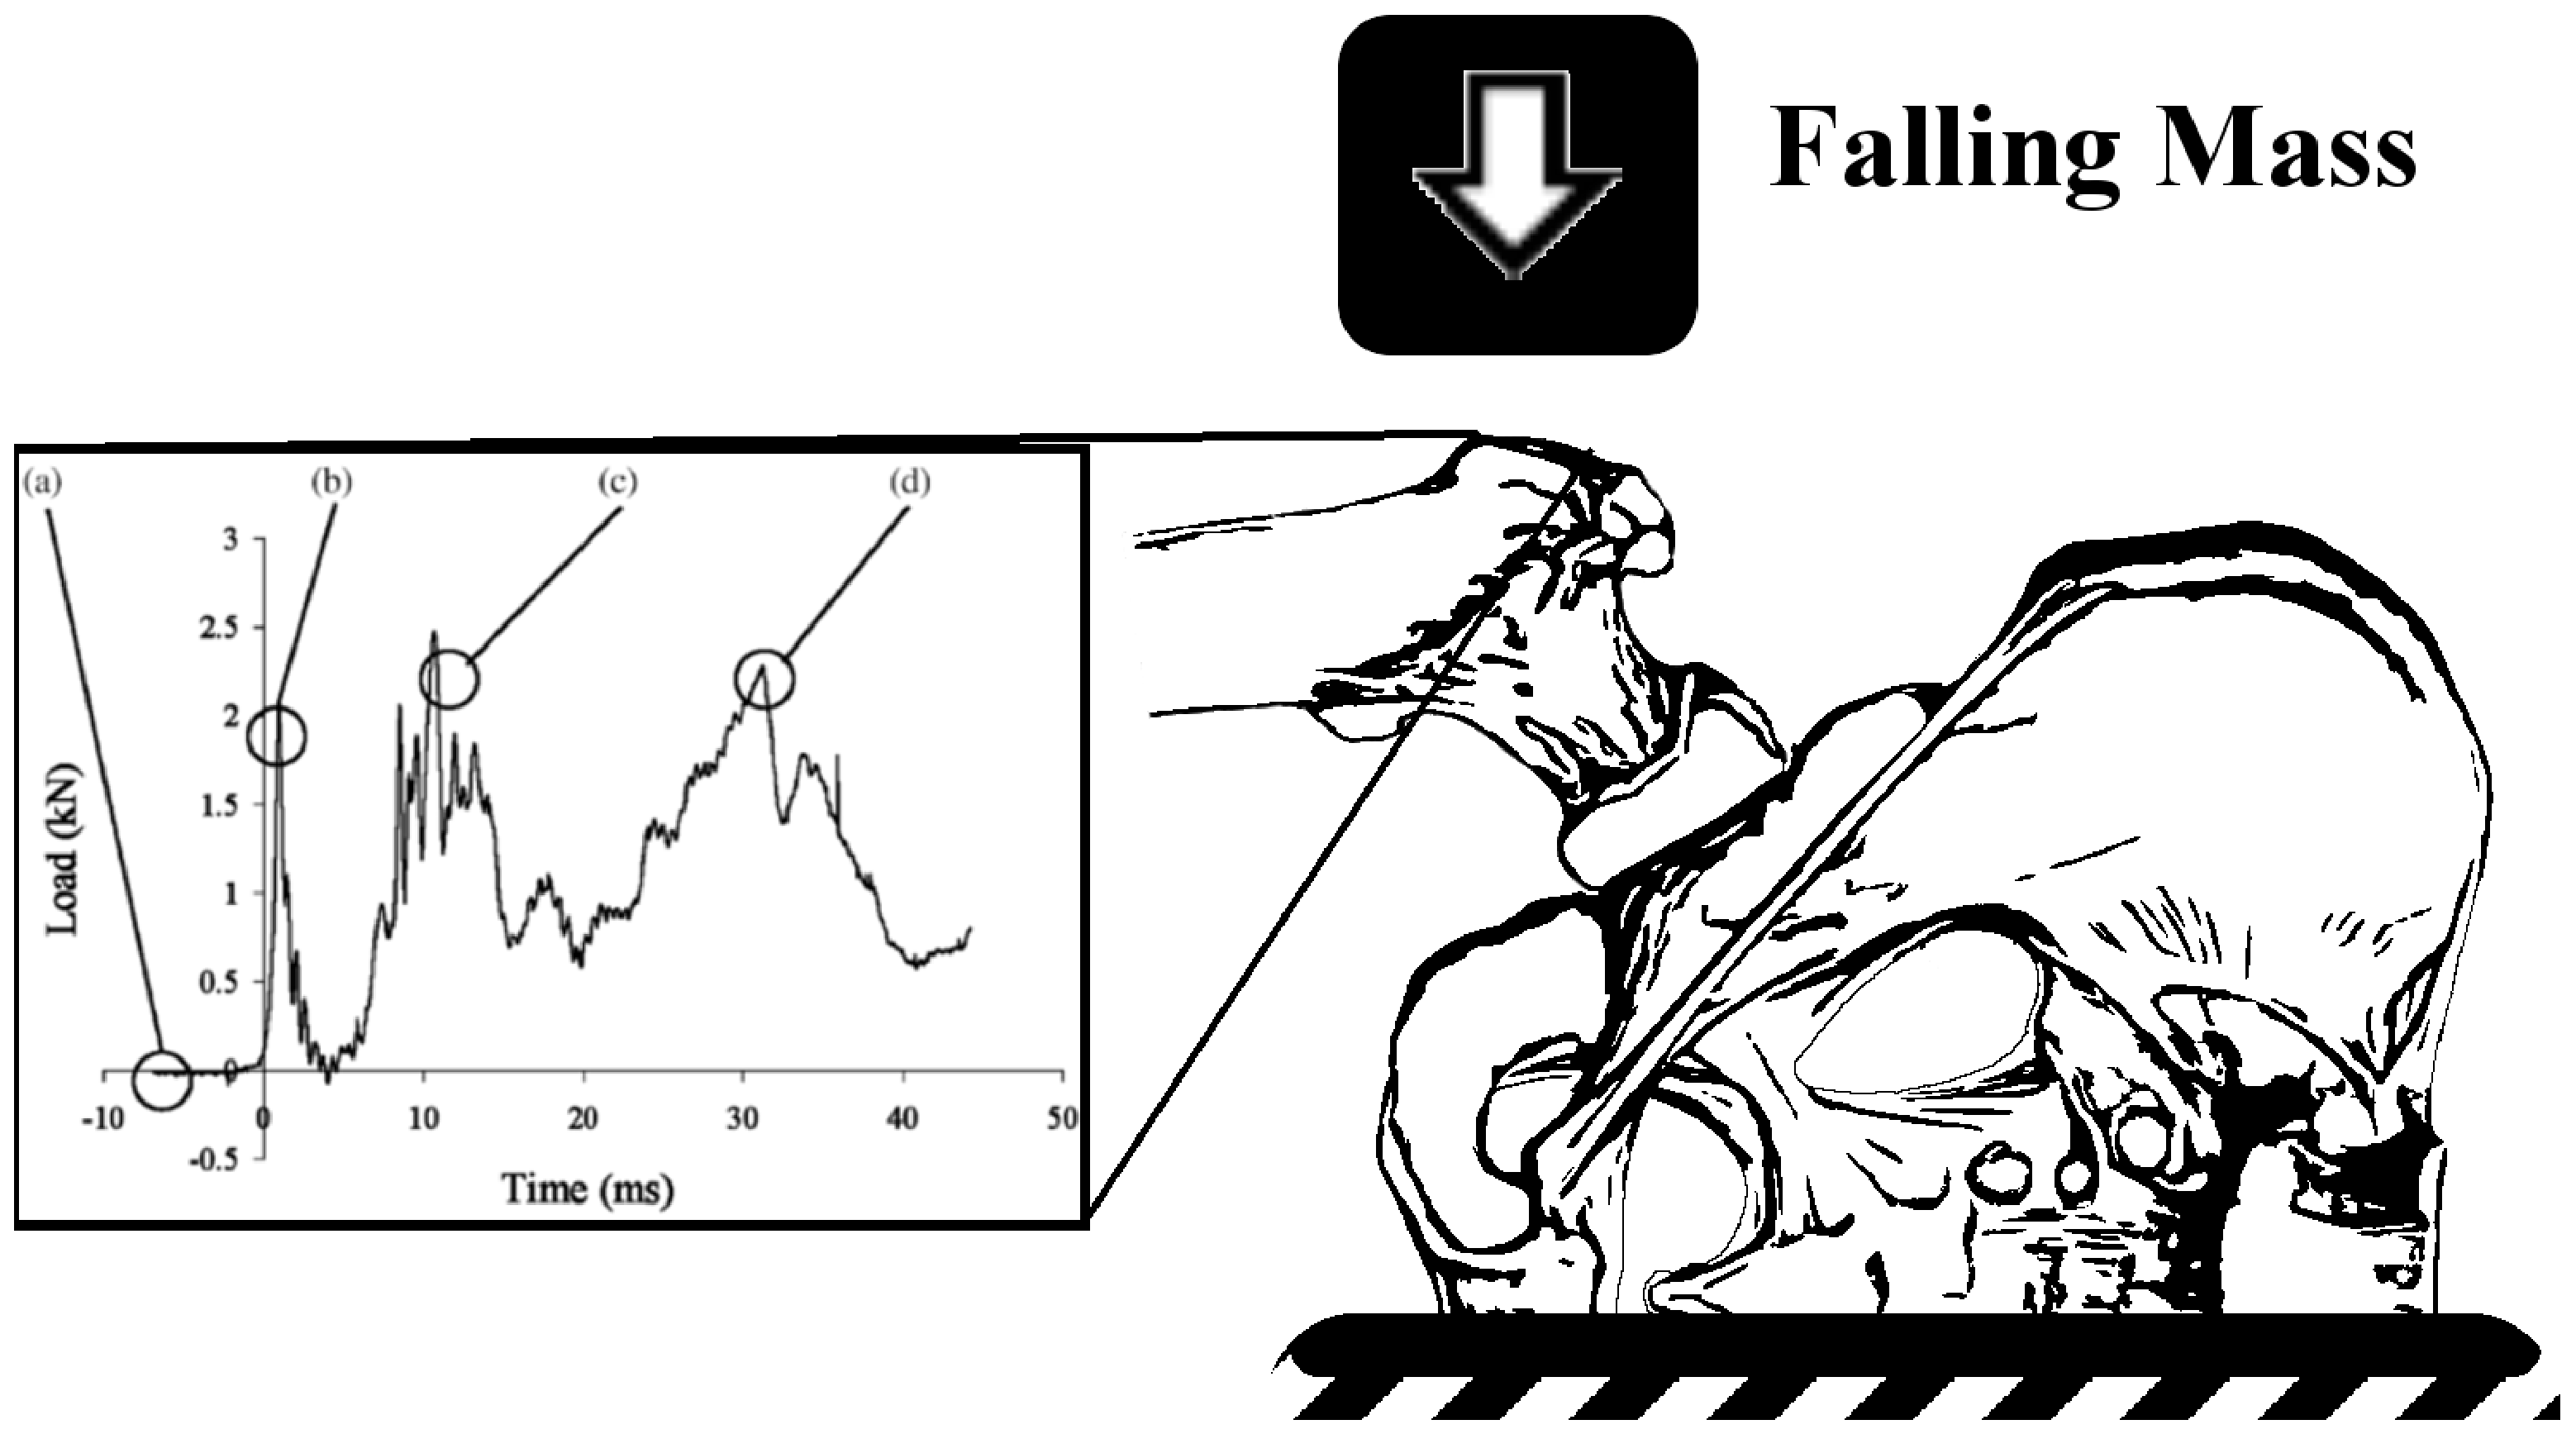
\includegraphics[width=1\linewidth]{./impactor/figures/BeasonComparison}
			\caption[Explanation of femur and lateral pelvis mass]{\textbf{In previous tests on osteoligamentous pelvises an instrumented impactor was dropped on the greater trochanter at 4.5~\ac{m}/\ac{s}.
			When the impactor came into contact with the trochanter a force spike was seen before deformation of the pelvis had begun, as indicated by peak (b) in the inset graph (adapted from \citet{beason_bone_2003}, with permission).
			This spike was created by the acceleration of the mass of the lateral pelvis and femur.}
			Illustrations adapted from \citet{gray_anatomy_1918}, copyright expired.}
			\label{fig:CompBeason}
		\end{figure}
		
		In the current apparatus, $m_{(eff\_p+f)}$ impacts a platen that is rigidly attached to a component used to hold and stabilize other parts of the apparatus (Figure \ref{fig:MassModel}).
		The mass of this stabilizing component influences the impulse delivered to the bone, and as such, the final value of $m_{(eff\_p+f)}$ needed to be tailored to the apparatus.
		The \textit{ex-vivo} value determined from the momentum analysis described above was used as a starting point for this process, and the mass was increased incrementally until the force delivered by the impulse matched a published, impact-velocity scaled, human volunteer test~\citep{laing_characterizing_2010}.
		The impact-velocity scaling was done by multiplying the human test by the ratio of (current experiment impact velocity)/(volunteer experiment impact velocity) which can be shown to be effective using impulse and vibration analysis.
		The final value for the pelvis mass was 1.98~\ac{kg}.

		\subsubsection{Pelvis stiffness}
		\label{sec:fall_sim_design_methods_apparatus_stiff}
		The pelvis has a finite stiffness, the value of which determines the duration of the impulse delivered by the effective body mass.
		This stiffness is not only a function of bone structure, but also body position at impact~\citep{robinovitch_distribution_1997, van_den_kroonenberg_hip_1996}, which must be taken into account when selecting the stiffness.
		Human volunteer experiments to characterize the stiffness of the pelvis~\citep{robinovitch_prediction_1991, robinovitch_distribution_1997, laing_characterizing_2010} have measured values ranging from 20.9 to 90~\ac{kn}/\ac{m}, depending on experimental protocol, and have shown its value to be constant above a compressive force of 300~\ac{n}~\citep{robinovitch_prediction_1991, laing_characterizing_2010}.
		Researchers used vibrational mechanics with various boundary conditions to determine the effective body mass and lateral stiffness of the pelvis~\citep{robinovitch_distribution_1997,laing_characterizing_2010} of human volunteers.
		The value of the effective body mass derived from one experimental condition~\citep{robinovitch_distribution_1997} was 32.8~\ac{kg}, which is similar to the effective body mass selected for the current experiment, and the corresponding pelvic stiffness was 35.4~$\pm$14.7~\ac{kn}/\ac{m}.
		This was selected as a base value for the current experiment, and was then modified to account for body position during the impact.
		
		Videos of volunteers falling have shown that people flex their trunks away from the ground at impact~\citep{van_den_kroonenberg_hip_1996, feldman_reducing_2007}, which increases the stiffness of the pelvis~\citep{robinovitch_distribution_1997}.
		To account for this, a spring with a rate of 50~\ac{kn}/\ac{m} was selected, corresponding to one standard deviation above the average stiffness for our base condition.
		The value of 50~\ac{kn}/\ac{m} also agreed with the recommendations of the international consensus statement for hip protector testing~\citep{robinovitch_hip_2009}.
		
		With the afore mentioned effective body mass and pelvis stiffness, the maximum anticipated deflection of the pelvis spring was 8~\ac{cm}.
		A steel spring with an outside diameter of 10~\ac{cm}, a free length of 35~\ac{cm}, and a maximum linear deflection of 18.6~\ac{cm} was used.
		A ratchet system with a tooth spacing of 9~\ac{mm} was incorporated to prevent rebound, as return of the stored energy post test was undesirable.

		\subsubsection{Soft tissue model}
		\label{sec:fall_sim_design_methods_apparatus_soft}
		Soft tissue over the greater trochanter is thought to protect the hip and prevent fractures in a sideways fall~\citep{majumder_effects_2008, robinovitch_prediction_1991, robinovitch_force_1995}.
		Researchers have shown that increasing the thickness of the soft tissue increases its ability to absorb and dissipate energy, thereby decreasing the potential for hip fracture.
		Computational work~\citep{majumder_effects_2008} showed a power-law relationship of $ Impact \; force \propto Thickness^{-0.2011}$.
		Experimental results from volunteer pelvis drop tests also showed a power-law trend of decreasing peak force with increased soft-tissue thickness, with a Spearman's $\rho$ = -0.71~\citep{robinovitch_prediction_1991}, and results from impact tests of cadaveric soft tissue~\citep{robinovitch_force_1995} showed that a 1~\ac{mm} increase in soft tissue thickness related linearly to a decrease in peak force of 70~\ac{n}.
		In the latter experiments, peak forces exceeded typical fracture forces for the proximal femur even for their highest tissue thickness of 45~\ac{mm}.
		
		Despite this understanding of how soft tissue attenuates impact force, epidemiological evidence of the protective nature of soft tissue is limited.
		Studies that have investigated the thickness of the soft tissue over the greater trochanter in fracture cases~\citep{bouxsein_contribution_2007, nielson_trochanteric_2009, minns_are_2007} have provided a pooled average and standard deviation of 29.4$\pm$15.6~\ac{mm}.
		Only a single study investigated the mechanical properties of the trochanteric soft tissue~\citep{laing_force_2008}, and showed that, while the stiffness of the tissue in the hip region of elderly individuals varied greatly with measurement location, they were typically around 20--35~\ac{kn}/\ac{m} over the greater trochanter when measured at a compressive stress of 100--140~kPa.
		
		For use in our fall simulator, a thickness one standard deviation below the average of fracture cases was selected in order to model an at-risk person.
		Due to material thickness availability, a final thickness of 19~\ac{mm} (0.75~inch) was chosen.
		This value also falls within the range recommended in the standardized hip protector testing protocol~\citep{robinovitch_hip_2009}.
		The material chosen had a stiffness of 26.5~\ac{kn}/\ac{m} at 95~kPa compressive stress (Evazote, Zotefoams Plc, Croydon, England), which was in the range of stiffnesses measured experimentally in the trochanteric region~\citep{laing_force_2008}.

		\subsubsection{Impact velocity}
		\label{sec:fall_sim_design_methods_apparatus_velocity}
		Impact velocity during a fall from standing is governed by two things.
		Firstly, the height of the person falling~\citep{van_den_kroonenberg_dynamic_1995}, and secondly any reactions, such as extending an arm to break the fall~\citep{feldman_reducing_2007}.
		Computational models~\citep{van_den_kroonenberg_dynamic_1995} of falls from standing have put the impact velocity at between 3.35 and 4.34~\ac{m}/\ac{s}.
		These values are higher than those observed in experimental tests where volunteers impacted their hips at a mean$\pm$SD of around 3$\pm$0.6~\ac{m}/\ac{s}~\citep{feldman_reducing_2007, van_den_kroonenberg_hip_1996}.
		
		An impact velocity of 3.0~\ac{m}/\ac{s} was selected based on the average of the volunteer tests~\citep{feldman_reducing_2007}.
		The specimen was placed stationary in the fall simulator (fall posture described below) and the effective body and pelvis+femur mass was dropped onto it.
		The effective body mass impacted the top of the pelvis spring, while $m_{(eff\_p+f)}$ bypassed the spring and contacted loading platens connected to the specimen through the soft-tissue model.
		To time these events so that they occurred coincidentally, $m_{(eff\_p+f)}$ was separated into two equal parts and suspended from the effective body mass by linear guide rods of length equal to the free length of the pelvis spring (Figures \ref{fig:MassModel} and \ref{fig:DT_setup}).
		This arrangement ensured that $m_{(eff\_p+f)}$ delivered a shock load at impact, and the effective body mass delivered a load mediated by the pelvis spring.

		\subsubsection{Specimen placement}
		\label{sec:fall_sim_design_methods_apparatus_placement}
		The surrogate bone was placed in the literature standard orientation for a fall to the side from standing.
		This orientation was, 10$^\circ$ adduction of the shaft and 15$^\circ$ internal rotation of the neck~\citep{courtney_effects_1994, de_bakker_during_2009, manske_cortical_2008, lochmuller_mechanical_2002}.
		Polymethylmethacrylate (PMMA, Bosworth Co, Skokie, IL) was used to make caps for the femoral head and lateral greater trochanter to prevent local crushing and also to provide even mounting surfaces.
		Each cap consisted of 20~\ac{g} of PMMA, formed by hand into a disk approximately 3.5~\ac{cm} in diameter, and moulded so that the head and trochanter loading surfaces were parallel.
	
	\subsection{Data collection and processing}
	\label{sec:fall_sim_design_methods_data}
	A six-axis load cell (Denton 4366J, Humanetics, Plymouth, MI), with an axial force capacity of $\pm$13.34~\ac{kn}, and non-linearity of $<$130~\ac{n}, recorded loads on the greater trochanter, between the pelvis spring and the specimen.
	
	Displacements of the greater trochanter and impact hammer were measured using a high speed video camera (Phantom v9, Vision Research, Wayne, NJ) imaging at 9216 frampes per second (fps) and a resolution of 576x288~\ac{px} (spatial resolution of 5~\ac{px}/\ac{mm}).
	Displacements were calculated from the video data using TEMA Automotive (v3.0, Image Systems, North Hollywood, CA).
	To determine the accuracy of this measurement, a validation study was carried out in which a bone surrogate (model 1130-21, Sawbones, Vashon, WA) was moved in a cyclic manner in the field of view of the displacement measurement camera.
	A dial gauge was recorded showing the displacement of the surrogate at any given time, and the results of the TEMA calculations were compared to the dial gauge at randomly selected times.
	The uncertainty of this measurement was determined to be $\pm$0.043~\ac{mm} ($\pm$\ac{sd}).
	
	Forces were recorded using a PCI-6040E (National Instruments, Austin, TX), 12~bit data acquisition board, and custom LabView software at a sampling rate of 20~\ac{khz}, with hardware anti-aliasing filtering at 10~\ac{khz}.
	The load cell outputs were amplified such that voltage saturation was attained at $\pm$6~\ac{kn}, giving a force resolution of 3~\ac{n}/bit.
	Imaging data was synchronized by recording a camera trigger signal generated by the drop tower gantry closing a switch as it fell.
	
	All data were forward and reverse, low-pass filtered using MatLab (2010b, The Mathworks, Natick, MA) with a -3~dB cut off at 500~\ac{hz}.
	Force data were processed with a fourth-order Butterworth filter and displacement data were processed with a second-order Butterworth filter.
	The cut off frequency of 500~\ac{hz} was chosen to remove high frequency ringing of the drop tower while retaining important impact events.
	The final fall simulator arrangement is shown in Figure \ref{fig:DT_setup}.
	
	\begin{figure}
		\centering
		\includegraphics[width=1.0\linewidth]{./impactor/figures/DT_setup2.eps}
		\caption[Photo of the fall simulator]{\textbf{A photo of the fall simulator showing each element of the model}}
		\label{fig:DT_setup}
	\end{figure}

	\subsection{Digital image correlation verification}
	\label{sec:fall_sim_design_methods_dic}
	A separate experiment was carried out to validate the use of \ac{dic} on the bone of the proximal femur for surface strain measurement.
	Subsequent tests in the fall simulator will use \ac{dic} strain measurement exclusively.
	
	Twenty human femoral specimens (3 normal, 11 osteopenic, 6 osteoporotic) were cleaned of soft tissue and periosteum, and a strain rosette (FRA-2-11-3LT, Tokyo Sokki Kenkyujo Co., Tokyo, Japan) was glued on the anterior-superior femoral neck using cyanoacrylate and a standard protocol~\citep[Chapter:~Strain gauge analysis of hard tissues: factors influencing measurements]{little_experimental_1992}.
	The femoral neck, including the strain gauge, of each specimen was painted with a white-on-black speckle pattern using an airbrush (VL, Paasche, Chicago, IL).
	The specimens were placed in a materials testing machine (8874, Instron, Norwood, MA) in the fall configuration~\citep{de_bakker_during_2009} discussed in \S\ref{sec:fall_sim_design_methods_apparatus_placement} and loaded to 50\% of their total aBMD predicted fracture load~\citep{boehm_prediction_2008}, at a constant compression rate of 0.5~\ac{mm}/\ac{s}.
	
	Force was output by the materials testing machine using a voltage scaling to provide 4~V at the target maximum load.
	Displacement was output with a constant scaling of 0.35~\ac{mm}/V.
	Three channels of strain data were collected at 20~\ac{khz} from the the strain rosettes using an SCXI-1520 strain gauge input module (National Instruments, Austin, TX) connected to the PCI-6040E, with hardware anti-alias filtering at 10~\ac{hz}.
	Two high speed video cameras (Phantom v12.1), recording at 100~fps and a resolution of 1280x800~\ac{px} (spatial resolution of approximately 17~\ac{px}/\ac{mm}), were used to observe the anterior-superior femoral neck including the strain gauge.	
	The video and voltage data were synchronized by recording the camera trigger signal which was emitted by the materials testing machine.
	The video images were imported into commercially available \ac{dic} software (StrainMaster, LaVison, G\"{o}ttingen Germany) for analysis.
	The \ac{dic} data were analysed using an iterative approach in which erroneous displacement vectors were identified as those that were \textgreater1.5~\ac{sd} from their immediate neighbours.
	These vectors were replaced by an average of their neighbours and reanalysed.
	After this second round of analysis, the strain field was filtered using a 3x3 median filter.
	The strain gauge data were taken as a gold standard measurement and the \ac{dic} data were compared to them in order to determine the \ac{dic}'s accuracy and precision.
	Comparisons were made using minimum principal strain since it is known to correlate to compressive failure~\citep{bayraktar_comparison_2004}.

\section{Results}
\label{sec:fall_sim_design_results}
The force-time profile of the fall simulator was compared to the same velocity-scaled human volunteer data discussed in \S\ref{sec:fall_sim_design_methods_apparatus_pelvis}.
The fall simulator and velocity-scaled human volunteer profiles were seen to be similar in timing and magnitude (Figure \ref{fig:CompareToLaing}).
The initial force peak in the fall simulator was 40\% higher than in the volunteer data and delayed by 5.2~\ac{ms}.
The average loading rate up to the initial peak was the same in both data sets, with a value of 122.4~\ac{kn}/\ac{s} in the fall simulator and 121.7~\ac{kn}/\ac{s} in the scaled volunteer data.
The force of the initial peak was observed to be increased by internal vibration of the pelvis spring, which can be seen as a sinusoidal variation throughout loading.
A Fourier analysis of the impact event showed that the amplitude of spring component was approximately 13\% of the dominant frequency component, however, its timing created a discrepancy in force equal to 80\% of the volunteer data at 16~\ac{ms} post impact.
The global peak force in the fall simulator was within 5~\ac{ms} of the volunteer data.
The rapid decrease in the fall simulator force after 50~\ac{ms} was due to the engagement of the ratchet, preventing rebound of the spring.

\begin{figure}
	\centering
	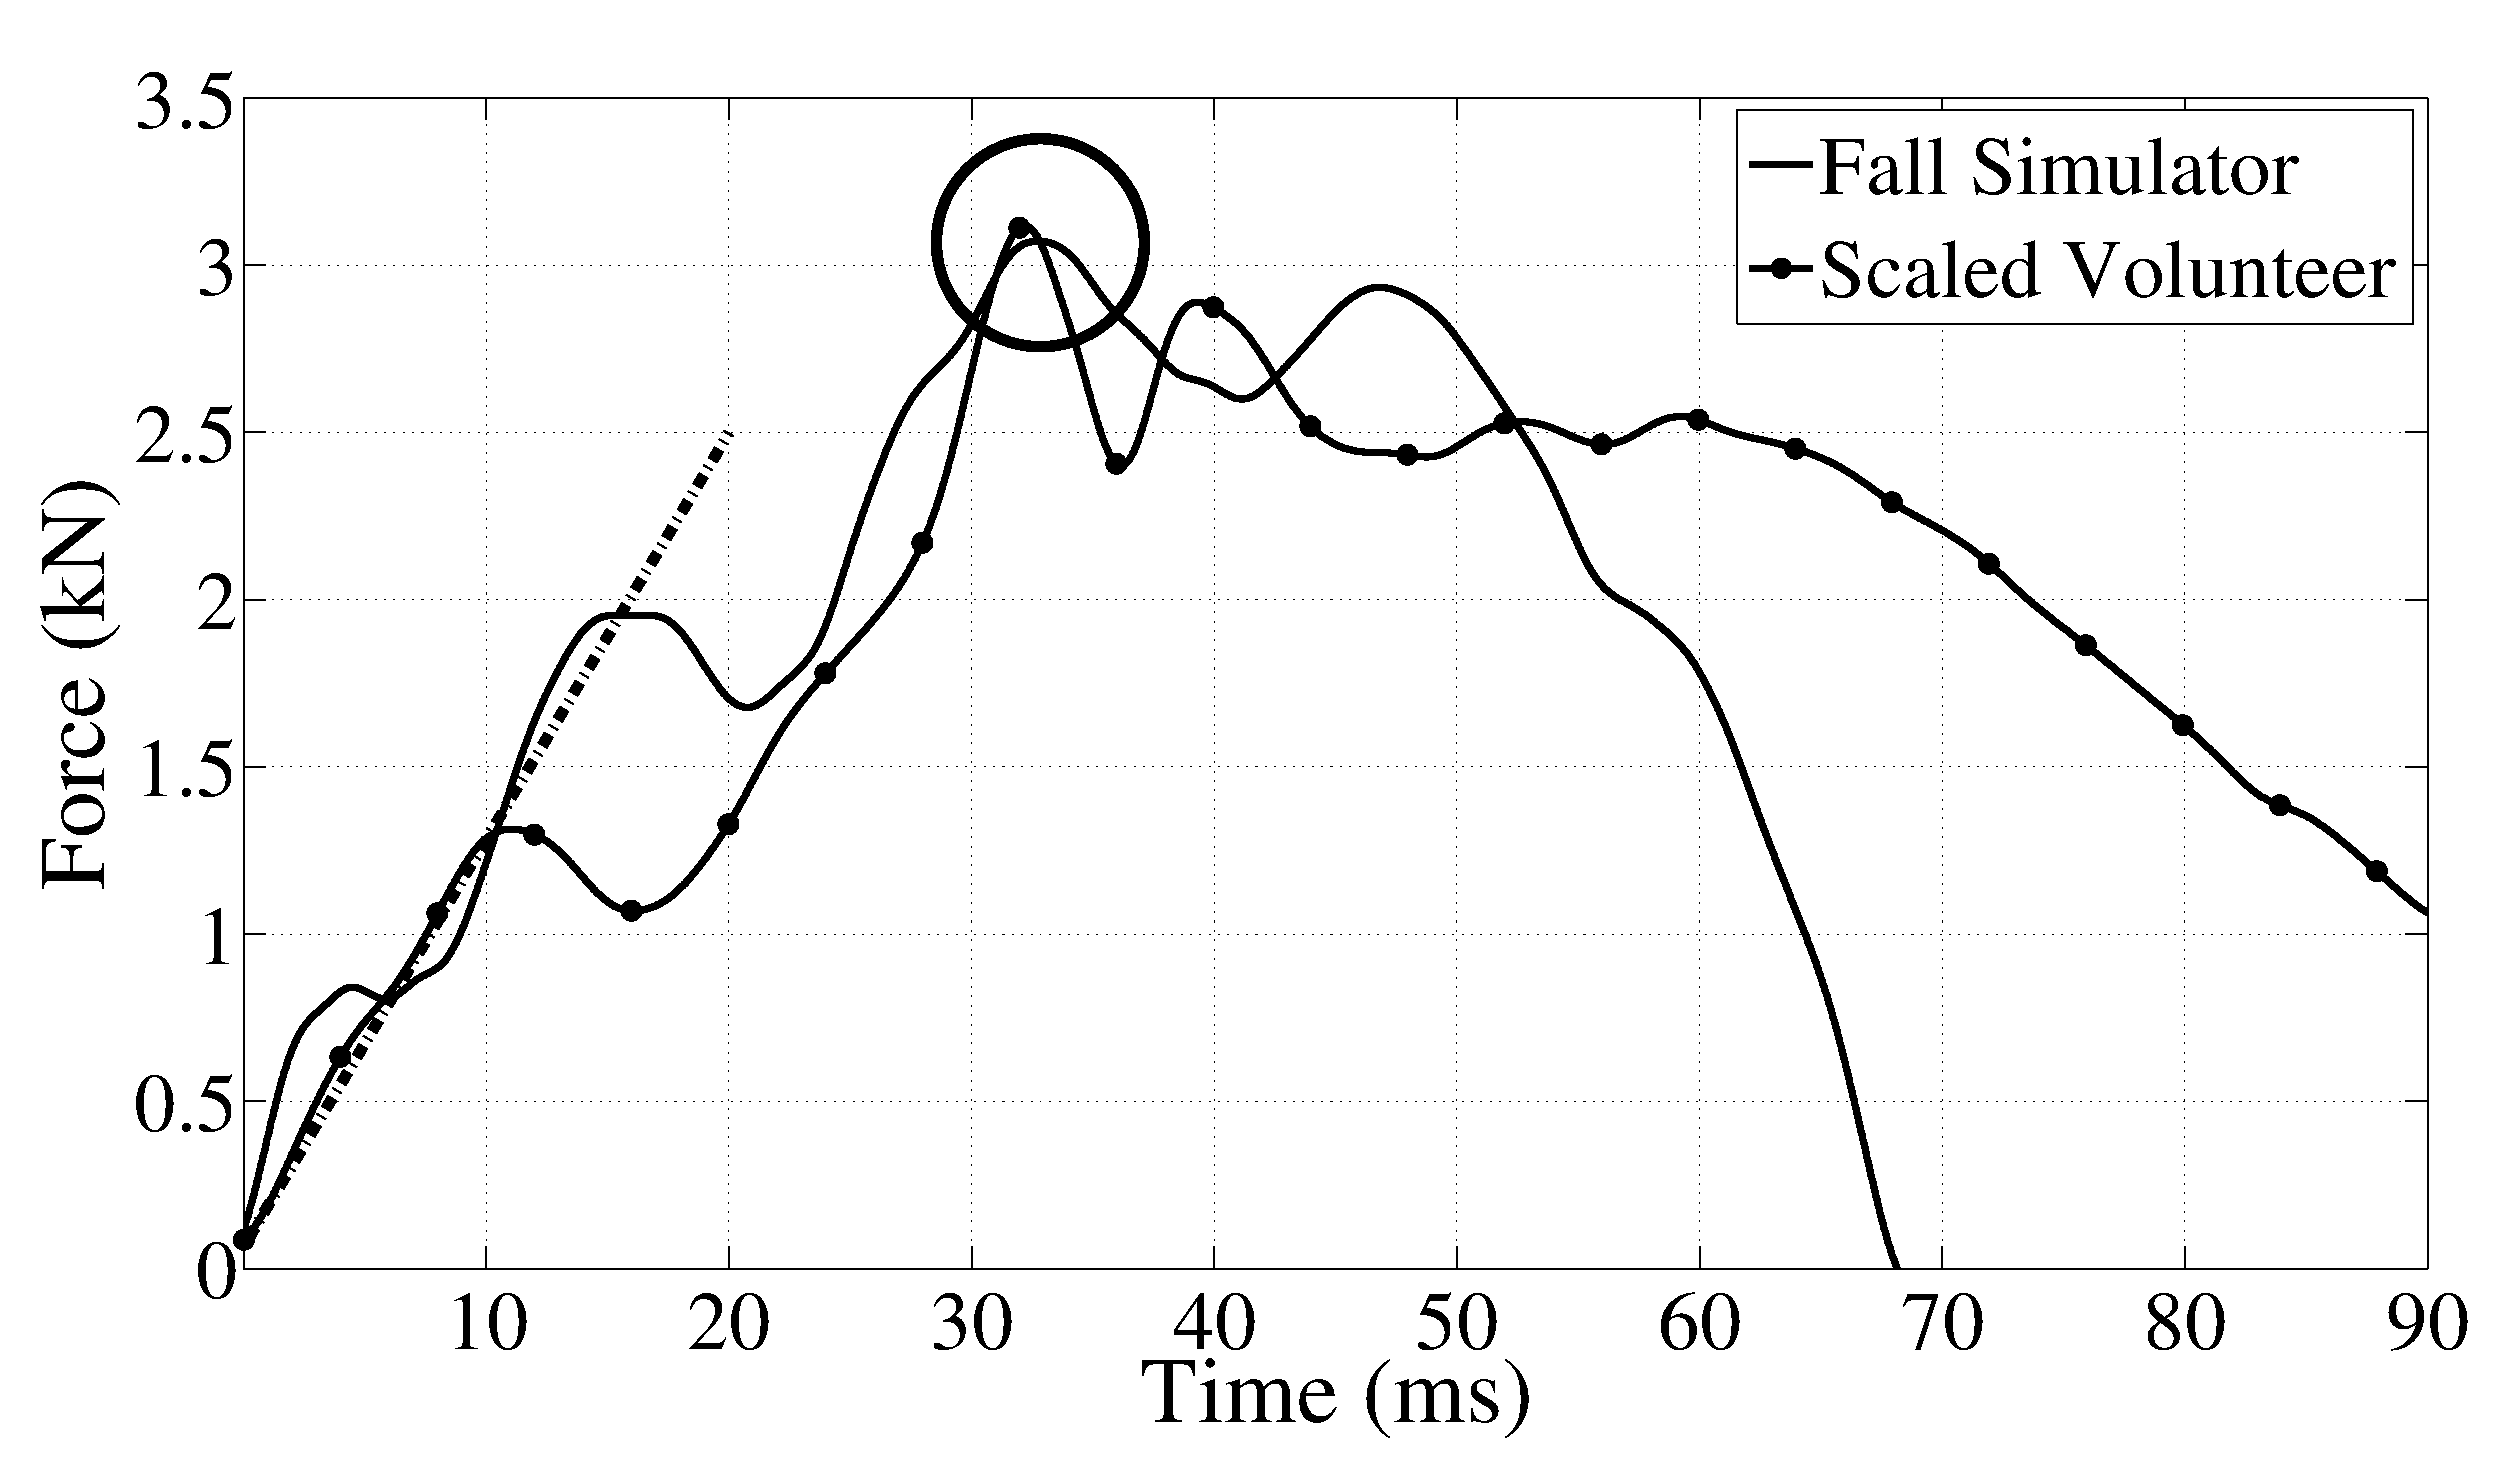
\includegraphics[width=1\linewidth]{./impactor/figures/CompareToLaing2010_VelocityScaled.eps}
	\caption[Fall simulator data compared to a human volunteer]{\textbf{An example response of the fall simulator plotted with human pelvis drop data~\citep{laing_characterizing_2010}.
	The dashed line indicates the initial loading slope of the scaled volunteer data and the circle indicates the location of the peak forces.
	The human data was scaled by the ratio of the impact velocities.}}
	\label{fig:CompareToLaing}
\end{figure}

In the \ac{dic} verification experiment, minimum principal strains from the \ac{dic} and the strain rosettes were well correlated (Figure \ref{fig:StrainErrors}).
The \ac{dic} result contained image-to-image noise (Figure \ref{fig:ExampleStrain}), the amplitude of this noise was found to be normally distributed and the frequency spectrum had no peaks in the range of 0-50~\ac{hz} (the Nyquist frequency), indicating that it was likely random in nature.
Three data sets (5, 8 and 10 in Figure \ref{fig:StrainErrors}) were subjected to camera vibration.
It is thought that one of the tripod legs was contacting the table supporting the materials testing machine, transferring vibrations associated with the hydraulic pump to the camera.
Identification of the faulty data sets was trivial, as strain would change by more than 1000~\ac{micro-eps} from frame to frame.
Excluding the datasets thus affected, the \ac{rms} average difference was 127~\ac{micro-eps} (range: [-375, 336]), and the standard deviation was 239~\ac{micro-eps}.

\begin{figure}
	\centering
	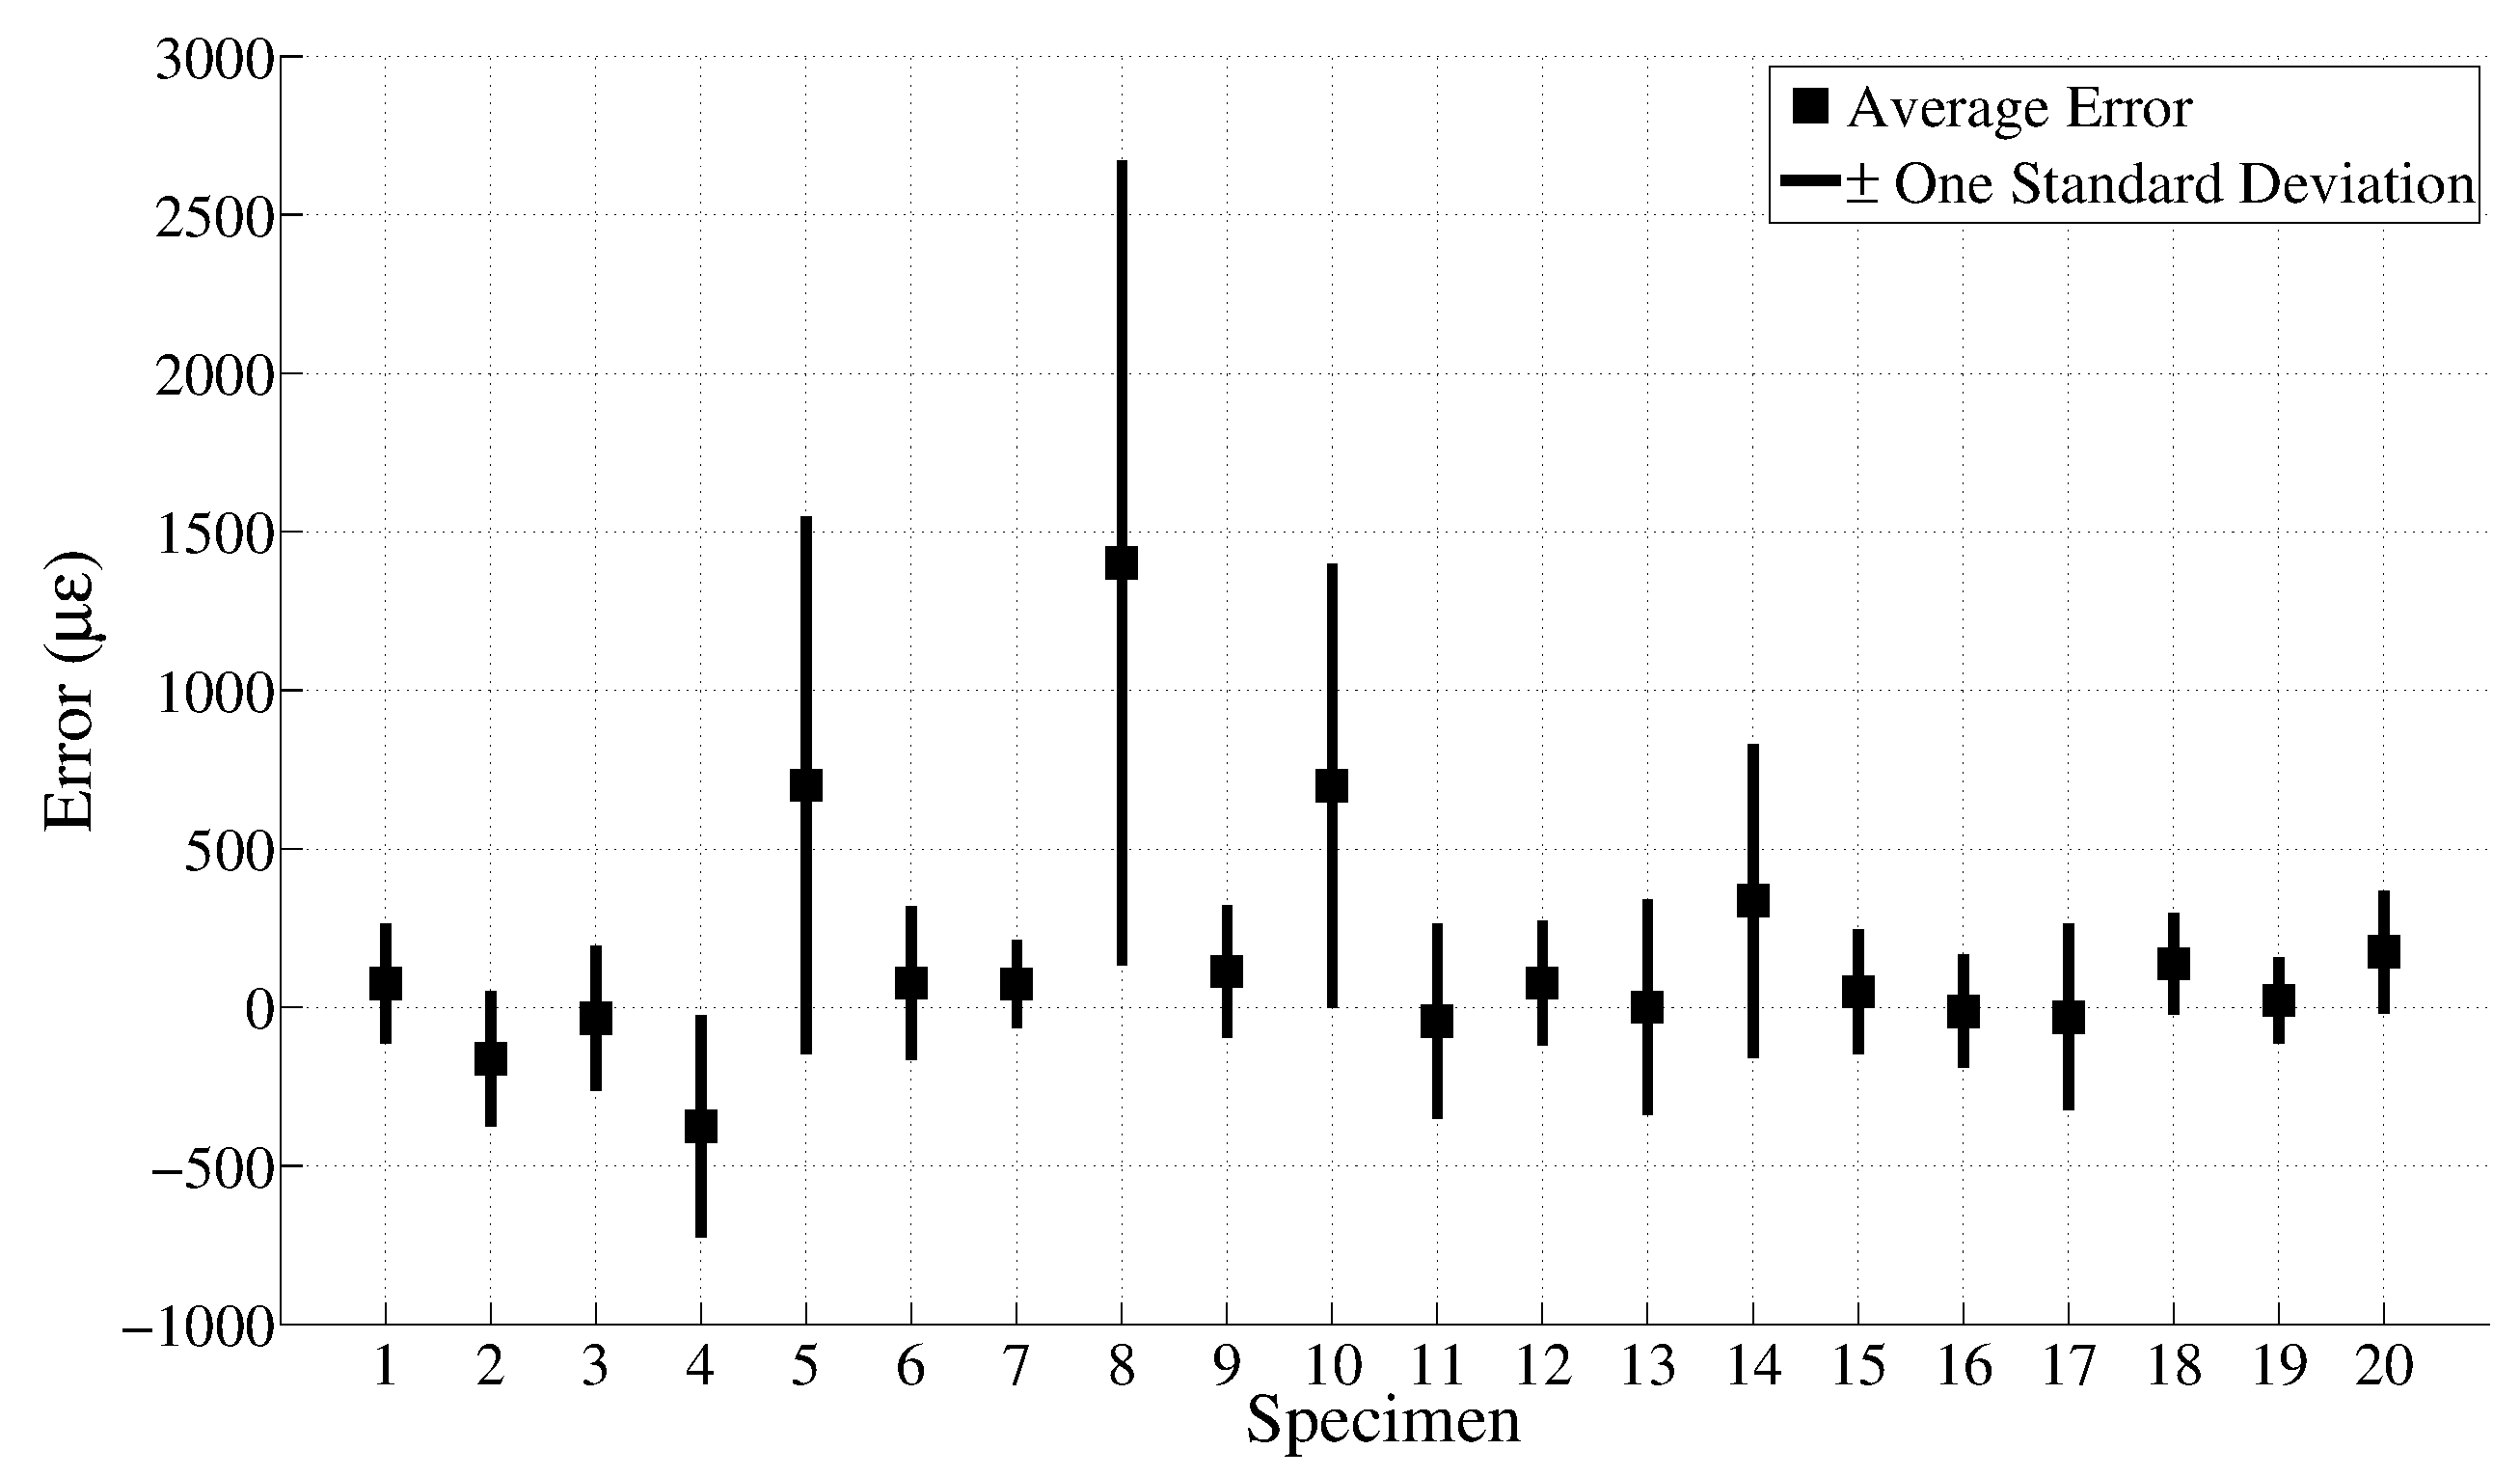
\includegraphics[width=1\linewidth]{./impactor/figures/StrainError.eps}
	\caption[Validation of \acf*{dic} on the femoral neck]{\textbf{The average and standard deviation of the strain errors measured for each specimen.
	Three specimens, 5, 8, and 10, were subjected to camera vibration, leading to incorrect \ac{dic} strain readings.}}
	\label{fig:StrainErrors}
\end{figure}

\begin{figure}
	\centering
	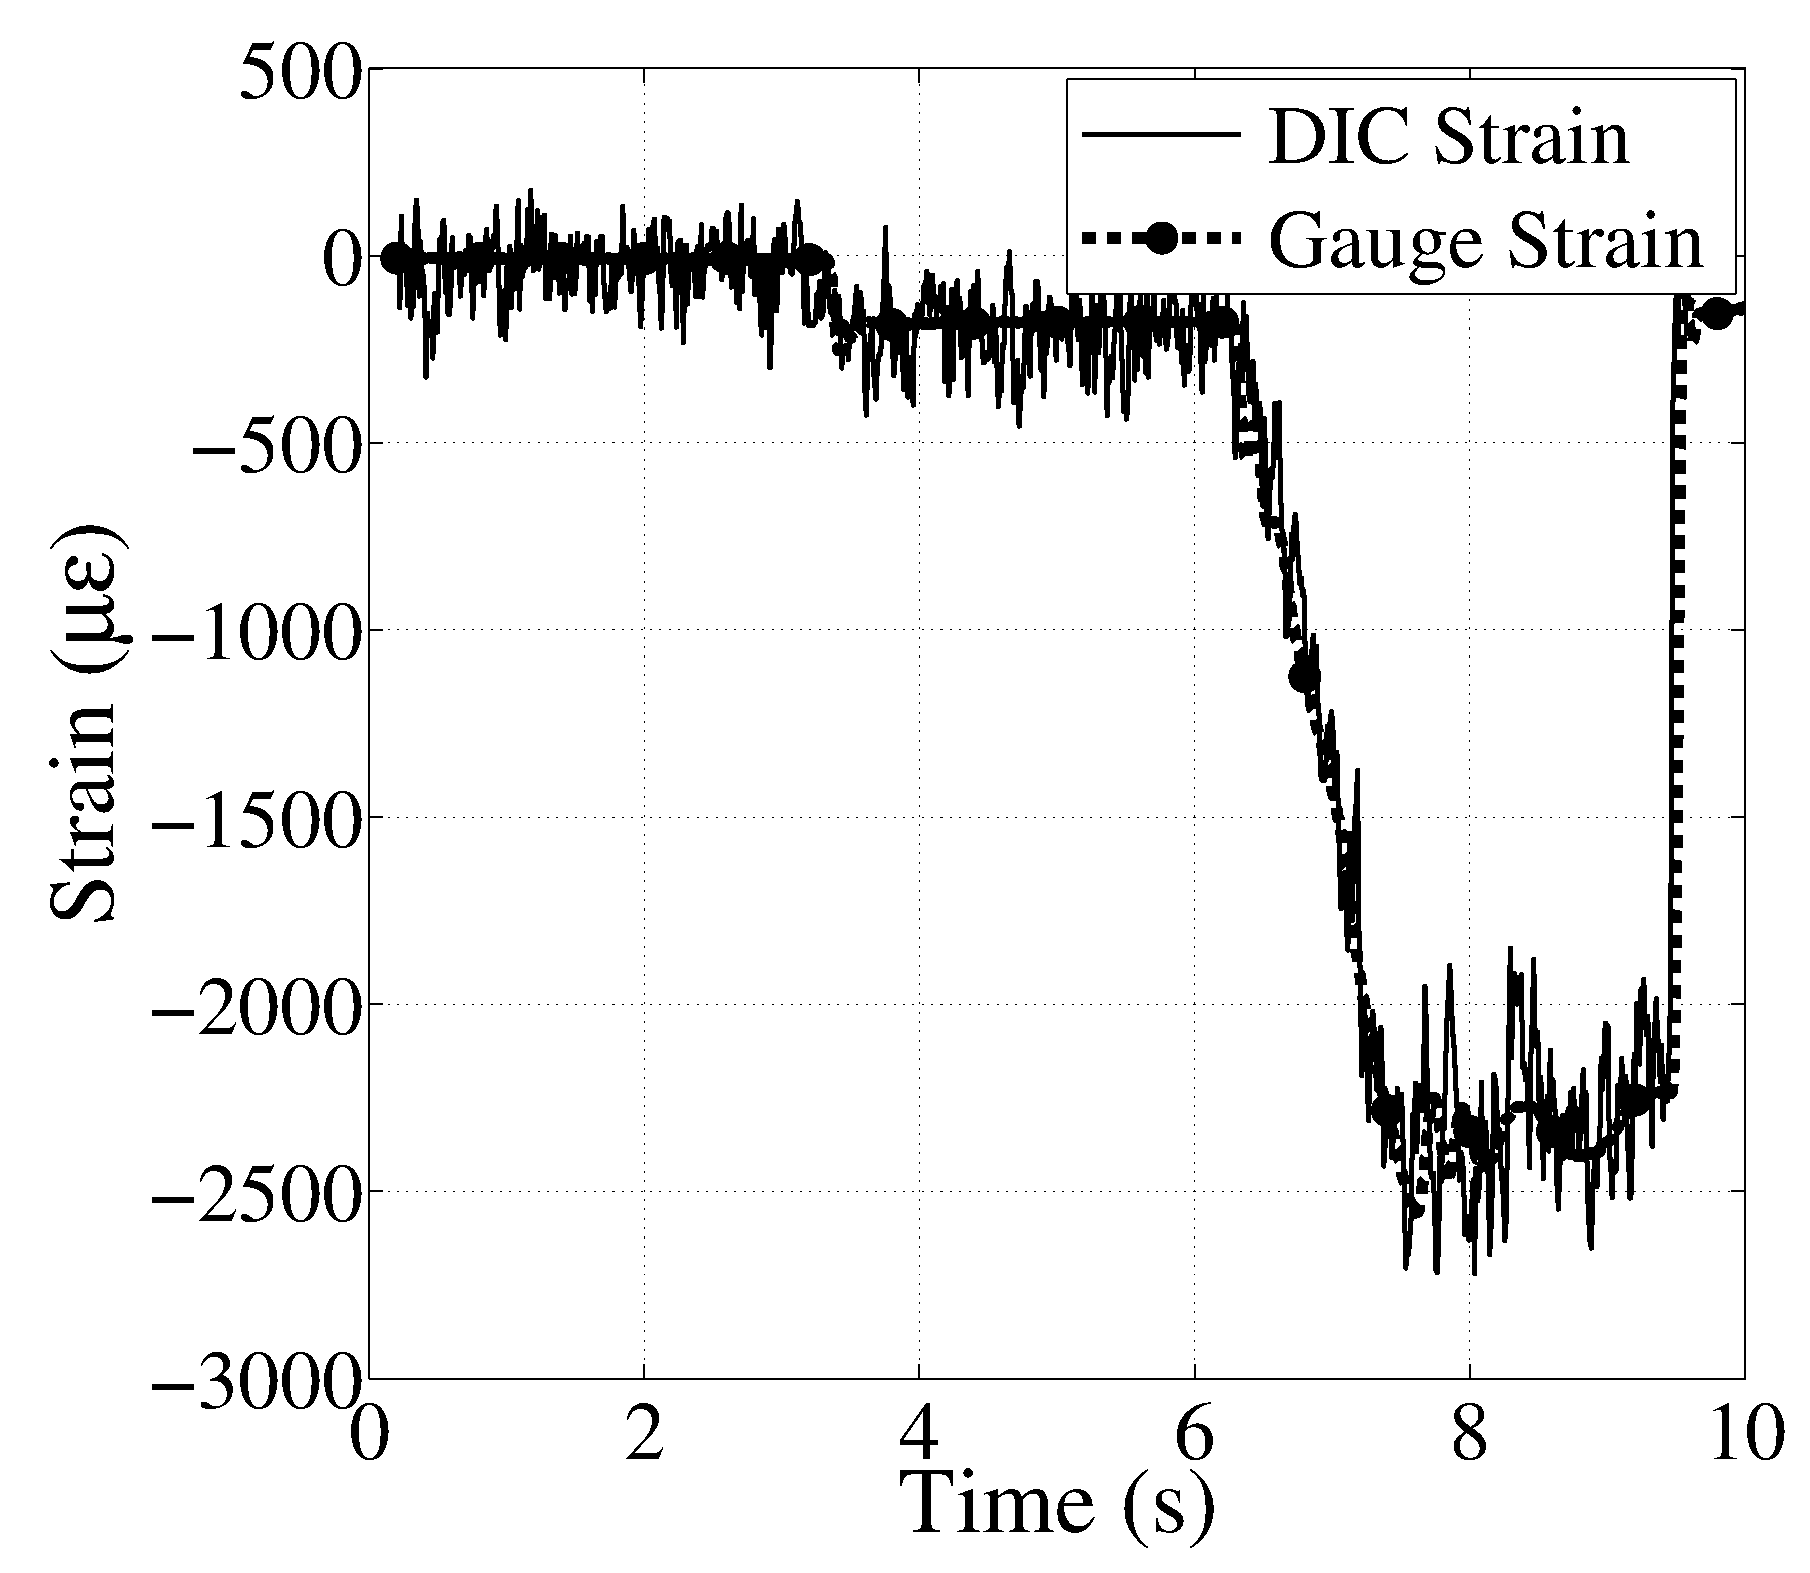
\includegraphics[width=0.7\linewidth]{./impactor/figures/StrainExample/StrainsTogether}
	\caption[Example \acs*{dic} strain and strain gauge data]{\textbf{Example data from the \ac{dic} analysis plotted with the strain gauge data. Time vs.\ strain plot for specimen 16 shows the character and magnitude of the random noise.}}
\end{figure}

\begin{figure}
	\centering
	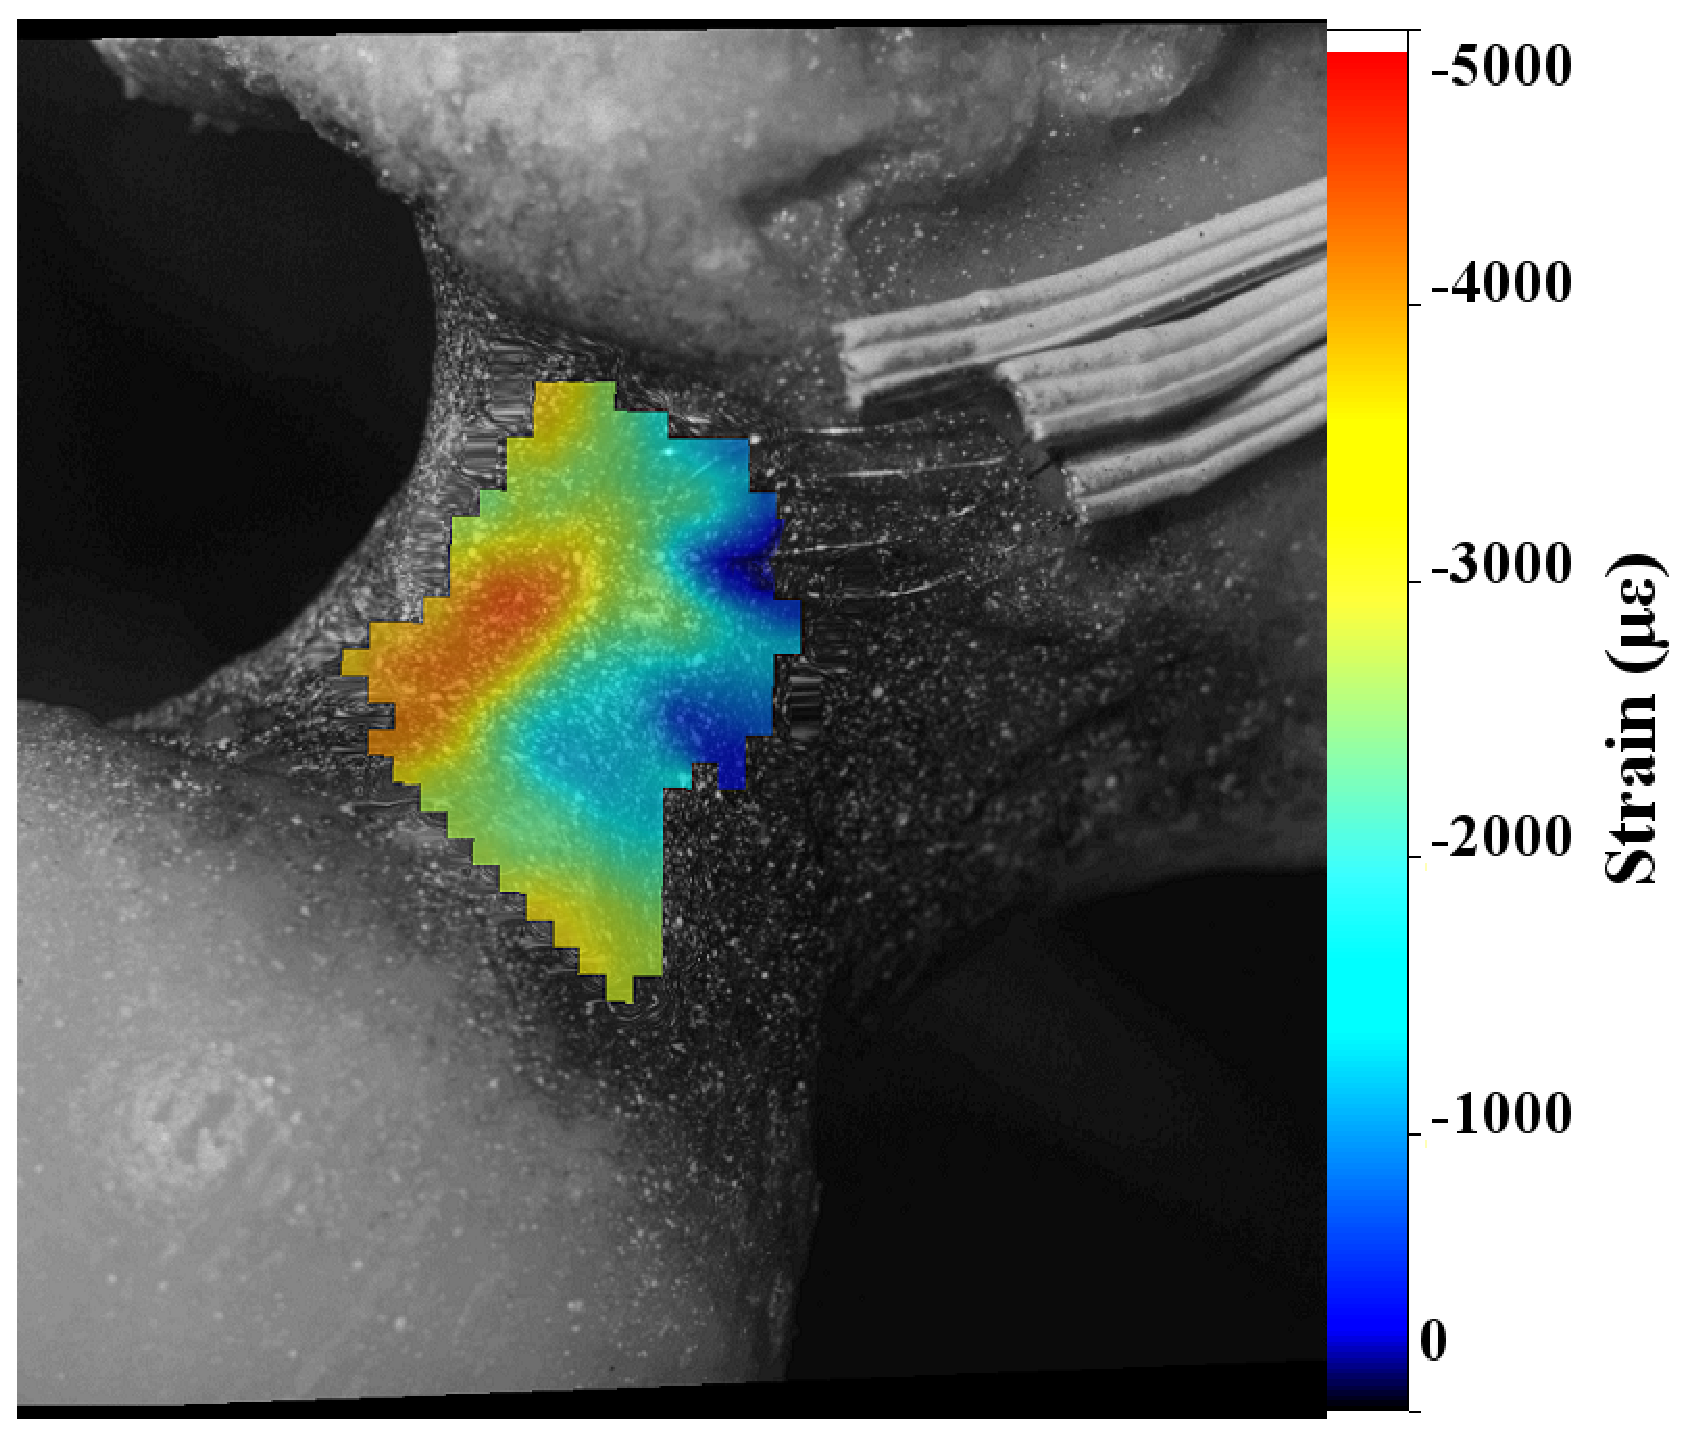
\includegraphics[width=0.7\linewidth]{./impactor/figures/StrainExample/H1376L_max_mod}
	\caption[Example surface strain data from the \acs*{dic} analysis]{\textbf{An example \ac{dic} strain contour map (b) shows how the strain varied over the surface of the bone at the maximum applied load. The bone is oriented such that superior is to the left and lateral to the top. The head of the femur is in the lower left and the trochanter occupies the upper portion of the image with the strain gauge wires visible on the right of the image.}}
	\label{fig:ExampleStrain}
\end{figure}

\section{Discussion}
\label{sec:fall_sim_design_discussion}
A method to simulate a fall to the side, impacting the greater trochanter of the femur, was developed.
A lumped parameter model of the human pelvis and hip joint, with the properties of each structure represented by literature values, was used.
Additionally, a method for full field strain analysis was validated on the neck of the proximal femur.

Previous researchers have developed models of the pelvis and body for use in hip protector testing~\citep{robinovitch_prediction_1991, robinovitch_hip_2009, laing_force_2008}, but a model appropriate for testing of cadaveric tissue has not been implemented.
The selected body mass and pelvis stiffness were similar to those selected by the previous researchers, which was reflected in the time to peak force being similar between our apparatus and theirs.
\citeauthor{robinovitch_force_1995}~\citep{robinovitch_force_1995, robinovitch_hip_2009} reported a time to peak force for their apparatus between 30 and 45~\ac{ms} post contact; our apparatus had a peak force at 32~\ac{ms}, with a plateau until $\sim$50~\ac{ms} due to oscillations of the pelvis spring.
The use of the ratchet to prevent rebound does not have an analogue in the previous literature because research on hip protectors used metal or plastic femur surrogates, which were not at risk of fracture during the test.
This change represents an adaptation required for testing of human material to obtain physiological fractures.

Another adaptation for physiological testing was changing the pelvis spring from mobile to stationary.
\citet{robinovitch_hip_2009} proposed two methods for fall simulation to test hip protectors, one of which used a moving linear spring, dropped in a drop tower similar to the current apparatus.
Our experiments using such an arrangement, in which the pelvis spring is dropped on the specimen, during the development of the current fall simulator, showed that the inertia of the spring's free-end was large enough to fracture a proximal femur before compression of the spring even began.
While the impulse due to the spring's mass may not be important for hip protector testing, which aims to attenuate the global force peak, it is important when testing cadaveric specimens.

One principal difference between the current fall simulator and the previous models, was the inclusion of the effective mass of the lateral pelvis and proximal femur.
Previous models neglected this mass and used signal filtering to remove artefacts created by shock loading and oscillations of the pelvis spring~\citep{robinovitch_force_1995, robinovitch_hip_2009}.
As discussed in $\S$\ref{sec:fall_sim_design_methods_apparatus_pelvis}, the impulse delivered by the effective mass of the lateral pelvis and proximal femur is physiologic and should be modelled.
This impulse creates a situation in the initial milliseconds of the impact of a high loading rate, which may change the behaviour of a human bone specimen in ways that are difficult to predict~\citep{mcelhaney_dynamic_1966, crowninshield_response_1974, robertson_compressive_1978, courtney_effects_1994, pithioux_comparison_2004, hansen_effect_2008, zioupos_microcracking_2008}.
The model showed that the magnitude of this impulse is determined more by the soft tissue mechanics than the stiffness of the bone.
A linear mathematical model of the current apparatus showed that the sensitivity of the impulse to the selected mass was low, with a 25\% increase in the mass changing the impulse magnitude by 6\%.
We believe that inclusion of this high loading rate portion of the curve may be important to gain an understanding of how the failure of the proximal femur is initiated and how it progresses.

The soft-tissue model in the current apparatus is minimal compared to those used in hip protector testing, in which researchers typically model the entire lateral trunk~\citep{laing_force_2008}.
Modelling of the trunk is a requirement for accurate fitting of the hip protectors but removes the possibility of observation of the femoral deformation.
The current apparatus required access to the femoral neck and trochanter for video observation.
A fall from standing might allow some of the energy to be dissipated to the surrounding tissues, however, an impact on the greater trochanter in a low BMI individual would likely have little energy dissipation into the surrounding tissues due to the prominence of the bony landmark.
Our fall simulator is modelling, in effect, the scenario that hip protectors are meant to address.

The impact velocity selected for the fall simulator was the average velocity from previously publish fall volunteer experiments~\citep{feldman_reducing_2007}.
This value is lower than the value of 3.4~\ac{m}/\ac{s} recommended by the international consensus statement on hip protector testing~\citep{robinovitch_hip_2009}.
The principal goal of the tests preformed for hip protector testing is to model a fall that would almost certainly create a fracture and see if it could be prevented through use of a biomechanical device.
The goal of the current research was not to model a severe fall, but to model a physiological fall that may, or may not result in fracture.
As mentioned in the introduction, previous hip fracture research tested all bones to failure.
The fall simulator described in this paper has the potential to identify bones that do not fracture in a fall to the side from standing, allowing further investigation of what is protective or detrimental to bone strength.

The orientation of the bone in the apparatus was selected based on preceding literature.
This placement is set by shaft angle from the vertical (adduction angle) and rotation of the neck (internal neck rotation).
Previous researchers selected the orientation by reviewing fracture studies and selecting adduction and neck rotation angles that created clinical fracture types~\citep{lotz_use_1990, backman_proximal_1957}.
The adduction angle was later modified to a more physiologic angle after video of human fall volunteers became available~\citep{courtney_effects_1994}.
The neck rotation angle has remained the same as it is difficult to evaluate its value in volunteers.
\Citet{feldman_reducing_2007} measured the angle of the contact point with the ground, around the circumference of the hip, in human volunteers who fell from standing height (the \emph{hip proximity angle}).
They found this angle to be an average angle of 8$^\circ$ posterior from directly lateral.
Combination of this value with the average femoral anteversion in the human population of 9.73$^\circ$~\citep{toogood_proximal_2009} gives an impact angle of 17.7$^\circ$, which is close to the and current value of 15$^\circ$.

Data processing for the current fall simulator differs from that proposed in previous work on hip protector testing.
Hip protector testing has used low pass filtering to clean unwanted artefacts from the signal by cutting off the signal at either 100~\ac{hz}~\citep{robinovitch_force_1995} or 50~\ac{hz}~\citep{robinovitch_hip_2009}.
The dynamics of the impulse delivered to the lateral trochanter, which we propose are seen by the proximal femur, are filtered out using such low cut-off frequencies.
We selected a value that retains the impulse at the trochanter and also retains the oscillations of the pelvis spring.
The filter cut-off frequency of 500~\ac{hz} provided us with a meaningful, but clean force-time trace, showing dynamical events that we believe are important to biofidelic modelling of physiologic falls to the side from standing.

Strain fields were obtained using \ac{dic} and verified at one location, using a triaxial strain rosette.
\ac{dic} has been used to measure the surface stains on porcine mandibles~\citep{yasuyuki_relationship_2009}, mouse tibiae~\citep{sztefek_using_2010} and on the surface of a plastic surrogate femur model~\citep{dickinson_experimental_2011}.
The magnitudes of strains measured on the mouse tibiae were compared with strain gauge measurements in similar locations on different specimens, but were not directly compared.
Due to the inhomogeneity of strain on the surface of the mouse tibiae, this comparison method has limited utility as a validation.
In the case of the plastic femur surrogate, \ac{dic} calculated strains were compared to a finite element model and found to agree in shape and magnitude.
However, the strain field on the plastic model was more uniform and did not display the high strain gradients seen in both our tests and those conducted on the mouse tibiae.
Our validation expanded upon both of these techniques by using a strain gauge, at the same time and location as \ac{dic}, to evaluate accuracy and precision of the \ac{dic} measurement on a human bone specimen.
The noise level of 230~\ac{micro-eps} is only 2.0\% of low rate yield strain, and 5.9\% of high rate yield strain of cortical bone in compression~\citep{hansen_effect_2008}.
Strain fields calculated by \ac{dic} in our experiments exhibited steep strain gradients, potentially due to the inhomogeneity of the bone in the human specimens.
This is similar to the strain fields seen in previous research~\citep{sztefek_using_2010}, and justifies the utility of \ac{dic} over point strain measurements.

We have developed a method to simulate a fall to the side from standing that addressed several limitations of previous fall models.
Our goal was to increase the biofidelity of physiologic fall modelling and we have included many aspects of the anatomy and impact that were previously omitted.
In light of these advances, there are notable limitations to discuss.
Firstly, the pelvis stiffness model included a spring which had a large mass and exhibited its own vibrations, influencing the overall loading pattern.
A number of different avenues for elimination of this artefact were investigated, including rubber dampening, as well as composite and elastomer springs.
Each of these came with its own limitations of either increasing the mass of the spring further, being difficult to characterize or being highly non-linear.
The limitation of a non-ideal spring (\ac{ie}, a spring with mass) is nearly impossible to eliminate, however, it was mitigated through the use of the ratchet system and by starting the test with the spring stationary.
We believe that the advantages of the drop tower method, namely free response of the specimen and biofidelic loading, outweigh the limitation imposed by the spring.
Secondly, the pelvis model lacks a damping element, which in life is the consequence of the soft tissues surrounding the pelvis.
Previous literature examined the potential range of damping of the pelvis and found a average value of 520$\pm$340~\ac{n}\ac{s}/\ac{m}~\citep{robinovitch_distribution_1997}.
Using fundamental vibrational mechanics, and our chosen mass, spring and initial velocity, inclusion of this damping would change the peak force by between 0.3\% and 6.3\%, with an average change of 2.2\%.
We believe this variation is acceptable in the context of human variability.
Third, the soft tissue model used in the current fall simulator is limited by the need to visualize the bone throughout the impact, and does not allow for transfer of force and energy to tissues that, in life, would surround the proximal femur.
In effect, our apparatus simulates individuals that are slender and have prominent trochanters, which are a target population for hip fracture prevention~\citep{nguyen_identification_2005}.
We feel the limitation of only modelling a subset of individuals based on soft tissue thickness is outweighed by the benefit of fracture visualization.
Fourthly, the impact model developed includes only the effective mass of the body that is active in the lateral direction.
In a fall to the side there are other important masses and inertias at play, namely the \ac{s-i} constraint on the femoral head by the mass of the body, and the rotational, mass, and friction constraints on the distal leg.
The \ac{s-i} constraint on femoral head will likely affect the final fracture lines produced more than the mechanical and failure behaviours of the bone.
Relaxed constraint of the lower leg would allow the orientation of the bone to change throughout the impact and could lead to different mechanical behaviours.
The added biofidelity of the latter change could lead to highly complex dynamics that would be difficult to analyse and reproduce, decreasing the consistency of the experimental boundary conditions.
Finally, fixed parameters for each of the elements in the apparatus reduces the ability to model a subject-specific fall for each femoral specimen.
A subject-specific design, allowing variation of the body mass, soft tissue thickness, and possibly, pelvis stiffness and $m_{(eff\_p+f)}$ would increase the biofidelity of the model.
However, the current level of understanding of how the parameters would vary based on body morphology is limited, and making appropriate changes would be difficult.
Additionally, changing all the experimental parameters in this manner would reduce the statistical power of a given set of experiments and greatly increase the required number of specimens.
The current arrangement of a set apparatus, with the only variable between experiments being the specimen, provides a way to identify specimens of interest in a manner that is efficient and statistically powerful.

Our method, which is driven by the energy of a free falling mass representing a person falling from standing, removes artificial imposition of trochanteric displacement rate and allows each specimen to deform based on local response and failure, permitting visualization of a specimen's physiologic failure progression.
In future experiments, we plan to test a multitude of specimens using this apparatus, characterize the fracture progression and compare the free response behaviour to the behaviour seen in previous fixed displacement rate experiments.
We believe that understanding how the mechanics change under dynamic loading will allow us to better understand hip fracture, eventually leading to improved prevention, detection and treatment of this debilitating condition.

